\documentclass[12pt,a4paper]{article}

\usepackage{caption}
\usepackage[utf8]{inputenc}
\usepackage[spanish]{babel}
\usepackage{url}
\usepackage{hyperref}
\usepackage{amsmath,amssymb,amsfonts}
\usepackage{graphicx}
\usepackage{float}
\usepackage{multicol}
\usepackage{xcolor}
\usepackage[left=2cm,right=2cm,top=2cm,bottom=2cm]{geometry}
\usepackage[authoryear]{natbib}
\usepackage{booktabs}
\usepackage{fontspec}
\usepackage{setspace}
\usepackage{tabularx}
\onehalfspacing
\setmainfont{Times New Roman}
\definecolor{azul}{rgb}{0.0, 0.53, 0.74}
\addto\captionsspanish{\renewcommand{\tablename}{Tabla}}

\title{El aislamiento y el enriquecimiento sensorial modulan de forma diferencial la polidipsia inducida por programa en ratas Wistar macho}
\author{Marcos Peña Sánchez-Covisa}
\date{2025}

\begin{document}

\begin{figure}[H]
    \raggedleft
    
\includegraphics[scale=0.05]{LogoUNED.jpg}
\end{figure}

\begin{center}
    {\Large \textbf{El aislamiento y el enriquecimiento sensorial modulan de forma diferencial la polidipsia inducida por programa en ratas Wistar macho}} \\
    \vspace{1mm}
    {\normalsize \textit{Isolation and sensory enrichment differentially modulate schedule-induced polydipsia in male Wistar rats}} \\
    \vspace{5mm}
    {\large Marcos Peña Sánchez-Covisa} \\
    \vspace{3mm}
    \textit{Facultad de Psicología, Universidad Nacional de Educación a Distancia}
\end{center}

\begin{center}
    \textcolor{azul}{\rule{150mm}{0.5mm}}
    \end{center}
    
    \vspace{3mm}
    
    \begin{center}
    \textbf{\large Resumen}
    \end{center}
    
    \begin{center}
    \begin{minipage}{0.9\textwidth}
    \noindent
    La polidipsia inducida por programa (PIP) es una conducta adjuntiva que surge bajo programas de reforzamiento intermitente y se ha propuesto como modelo de afrontamiento compulsivo. El presente estudio analiza cómo la privación social y el enriquecimiento sensorial interactúan en la expresión de la PIP. Treinta y dos ratas Wistar macho (ocho semanas) se distribuirán aleatoriamente en cuatro condiciones de estabulación: aislamiento sin estímulos sensoriales (A--ES), aislamiento con estímulos (A+ES), vida en grupo con estímulos (G+ES) y vida en grupo sin estímulos (G--ES). Tras catorce días de estabulación diferencial, los animales completaron veinte sesiones diarias de 60 minutos bajo un programa de tiempo fijo de 30 segundos (TF-30~s) de entrega de alimento. Se registraron lametones al biberón, entradas al comedero y cruces de zona.
    
    Esperamos que los resultados revelen un gradiente decreciente de PIP, con una mayor expresión en la condición de aislamiento sin estimulación sensorial, seguida por el aislamiento con estimulación, el grupo con estimulación, y la menor expresión en el grupo sin estimulación sensorial. Se anticipan efectos principales significativos tanto de la condición de estabulación como de la sesión, así como una interacción entre ambas. Se espera que la interacción social atenúe la PIP de forma más eficaz que la estimulación sensorial; esta última, en ausencia de compañía, parece potenciar la conducta.

    De confirmarse los resultados previstos, podría interpretarse que la PIP actúa como una estrategia de autorregulación frente a la privación socioemocional y que el enriquecimiento físico, aplicado a sujetos vulnerables, puede tener efectos paradójicos. Se discuten implicaciones para los protocolos de bienestar animal y para los modelos preclínicos de compulsividad, resaltando la necesidad de considerar el contexto social en la prevención de conductas desadaptativas.
    
    \vspace{2mm}
    \noindent
    \underline{\textbf{Palabras clave:}} \textit{modelo animal de compulsividad, autorregulación emocional, conducta adjuntiva, afrontamiento disfuncional}
    \end{minipage}
    \end{center}
    
    \vspace{5mm}
    
    \begin{center}
    \textbf{\large Abstract}
    \end{center}
    
    \begin{center}
    \begin{minipage}{0.9\textwidth}
    \noindent
    Schedule-induced polydipsia (SIP) is an adjunctive behaviour that emerges under intermittent reinforcement schedules and has been proposed as a model of compulsive coping. This study examines how social deprivation and sensory enrichment interact in the expression of SIP. Thirty-two male Wistar rats (eight weeks old) will be randomly assigned to four housing conditions: isolated without sensory stimuli (A--ES), isolated with sensory enrichment (A+ES), group-housed with enrichment (G+ES), and group-housed without enrichment (G--ES). After fourteen days of differential housing, the animals will undergo twenty daily 60-minute sessions under a fixed-interval 30-second (FI-30~s) food delivery schedule. Licking at the water spout, feeder entries, and zone crossings will be recorded.

    The expected results point to a descending gradient of SIP expression: highest in isolated animals without stimulation, followed by isolated animals with enrichment, then group-housed animals with enrichment, and lowest in group-housed animals without enrichment. Significant main effects of housing condition and session are anticipated, along with a meaningful interaction between both factors. Social interaction is expected to attenuate SIP more effectively than sensory enrichment; the latter, in the absence of conspecifics, may paradoxically amplify the behaviour.

    If confirmed, these findings would support the interpretation of SIP as a form of emotional self-regulation in response to socio-emotional deprivation, and suggest that physical enrichment, when applied to vulnerable individuals, can have paradoxical effects. Implications are discussed for animal welfare protocols and for the development of preclinical models of compulsivity, highlighting the importance of social context in the prevention of maladaptive coping behaviours.
    
    \vspace{2mm}
    \noindent
    \underline{\textbf{Keywords:}} \textit{animal model of compulsivity, emotional self-regulation, adjunctive behaviour, maladaptive coping}
    \end{minipage}
    \end{center}
    
    \vspace{3mm}
    
    \begin{center}
    \textcolor{azul}{\rule{150mm}{0.5mm}}
    \end{center}
       

\vspace{15mm}

\begin{multicols}{2}

\section{Introducción}

Las conductas inducidas por programa (CIP), también denominadas conductas adjuntivas, emergen cuando un reforzador se entrega de forma intermitente y provocan patrones excesivos que no guardan una relación instrumental directa con dicho reforzador. \citet{Falk1961} describió por primera vez que ratas con acceso libre a agua desarrollaban ingestas masivas inmediatamente después de cada entrega de comida; denominó a este fenómeno polidipsia inducida por programa (PIP).

Dos marcos teóricos principales han tratado de explicar la génesis de la PIP. \citet{Staddon1977} la interpretó como una respuesta desplazada que aflora en estados motivacionales intermedios, cuando la probabilidad de obtener el reforzador es contingente pero todavía lejana. Por su parte, \citet{Killeen2013} reformularon el problema desde la contigüidad temporal: la proximidad entre una respuesta protoadjuntiva y la entrega del reforzador bastaría para fortalecerla mediante reforzamiento operante, incluso en ausencia de contingencia causal.

La literatura muestra de forma relativamente consistente que el aislamiento social se asocia con un aumento en la probabilidad de aparición de conductas estereotipadas, incluida la polidipsia inducida por programa (PIP) \citep{Jones1989,ibias2016effects,wang2024social,GROSS201261}. Si bien en la literatura sobre bienestar animal las conductas estereotipadas y compulsivas suelen agruparse por su similitud formal —movimientos repetitivos, invariantes y resistentes al cambio—, conviene distinguir ambos constructos. Las estereotipias suelen emerger en contextos de restricción ambiental y carecen de una función clara, mientras que las compulsiones, aunque también repetitivas, se interpretan como intentos de afrontar estados de tensión o ansiedad. En este sentido, la PIP puede exhibir un patrón estereotipado, pero su valor reside precisamente en su posible función reguladora, lo que justifica su conceptualización como conducta compulsiva más que puramente estereotipada. Esta asociación suele interpretarse desde la premisa de que los entornos empobrecidos generan un estado emocional crónicamente alterado, lo que favorece la emergencia de patrones conductuales desadaptativos. En esta línea, \citet{GarciaRebollar2024} advierten que la falta de estimulación adecuada compromete tanto el bienestar como la integridad neurofisiológica, facilitando disfunciones y alteraciones conductuales. A partir de estos planteamientos, \citet{Moreno2012} proponen que la PIP puede concebirse como un modelo de compulsividad y, en particular, como una forma de afrontamiento frente a condiciones emocionalmente disruptivas, como la incertidumbre derivada de los programas de reforzamiento intermitente. La consideración de la PIP como conducta compulsiva se basa en varios rasgos que comparte con otros modelos de compulsividad en humanos y animales. En primer lugar, la conducta se manifiesta de forma excesiva, repetitiva y aparentemente desadaptativa, sin una relación instrumental clara con el reforzador. En segundo lugar, persiste a pesar de su escasa utilidad funcional y puede interferir con otras conductas adaptativas. Finalmente, su emergencia ha sido asociada a estados emocionales negativos y condiciones de estrés, lo que sugiere un componente de regulación afectiva. Estos criterios coinciden con las características clave de la compulsividad descritas en el contexto de trastornos como el trastorno obsesivo-compulsivo (TOC) o las adicciones, donde las conductas son reiteradas, difíciles de suprimir, y actúan como estrategias de afrontamiento disfuncionales frente al malestar emocional \citep{Fineberg2010}.

Desde esta perspectiva, cabría esperar que su expresión se modulase en función del estado emocional del animal y, por extensión, de variables contextuales como el entorno social o físico. Sin embargo, esta predicción no siempre se cumple. \citet{FuentesVerdugo2023} hallaron que ratas alojadas en condiciones enriquecidas —tanto física como socialmente— desarrollaban la PIP con mayor rapidez e intensidad que aquellas mantenidas en aislamiento. Este hallazgo sugiere que un entorno altamente estimulante podría incrementar la sensibilidad al contraste incentivo bajo programas intermitentes, facilitando respuestas excesivas en lugar de inhibirlas.

Una línea complementaria enfatiza la dimensión socioemocional de la compulsividad. \citet{MartinGonzalez2022} demostraron que ratas seleccionadas como altamente compulsivas mediante el paradigma de PIP presentan un perfil socioemocional alterado, caracterizado por una menor dominancia social en la prueba del tubo, una mayor resistencia a la extinción de la memoria emocional en la tarea de evitación pasiva y una respuesta atenuada del eje HPA. Estos resultados sugieren que la compulsividad no se manifiesta únicamente en patrones motores repetitivos, sino que también implica alteraciones emocionales y motivacionales más amplias, contribuyendo a definir un fenotipo compulsivo con componentes socioemocionales específicos.

El enriquecimiento ambiental tampoco es intrínsecamente protector. \citet{Branchi2006} reportaron que crías sometidas a un “nido comunal” —alta estimulación social temprana— exhibían mayor ansiedad en la edad adulta sólo cuando se evaluaban en soledad; la presencia de un congénere anulaba dicha hiperreactividad. Así, la interacción entre estimulación sensorial y disponibilidad social podría amplificar o amortiguar la activación emocional según el contexto.

Aunque diversos trabajos han abordado el papel del aislamiento social o del enriquecimiento ambiental por separado, son escasos los estudios que examinan su interacción de forma sistemática en relación con la PIP. La contradicción entre resultados que apuntan a un efecto protector del enriquecimiento y otros que sugieren una potenciación paradójica de la conducta compulsiva pone de relieve la necesidad de clarificar los mecanismos subyacentes. Esta ambigüedad limita la validez del paradigma como modelo de afrontamiento y plantea dudas sobre su aplicabilidad traslacional. En este sentido, el presente trabajo busca responder a una pregunta central: \textit{¿cómo interactúan el contexto social y la estimulación sensorial en la modulación de la PIP?} Al aportar un diseño que permite contrastar esta interacción de forma controlada, se espera contribuir a delimitar las condiciones bajo las cuales la PIP refleja una estrategia adaptativa frente al estrés o, por el contrario, una manifestación de vulnerabilidad emocional.

El objetivo de este estudio es examinar cómo interactúan la privación social y la estimulación sensorial en la modulación de la polidipsia inducida por programa (PIP), considerada un modelo de conducta compulsiva. Para ello, se empleará un diseño experimental factorial con cuatro condiciones de estabulación diferencial: aislamiento sin estimulación sensorial, aislamiento con estimulación sensorial, vida en grupo con estimulación sensorial y vida en grupo sin estimulación sensorial. Tras catorce días de estabulación, los animales completarán veinte sesiones diarias de 60 minutos bajo un programa de tiempo fijo de 30 segundos.

Se espera, en primer lugar, que la privación social incremente la expresión de la PIP, y que la estimulación sensorial, por el contrario, la reduzca. En segundo lugar, se anticipa una interacción entre ambas variables: la mayor intensidad de PIP se produciría en animales aislados sin estimulación sensorial, seguida por los aislados con estimulación, los alojados en grupo con estimulación, y finalmente, la menor expresión correspondería a los alojados en grupo sin estimulación sensorial.

Aunque la propuesta se circunscribe al nivel preclínico, dilucidar cómo el contexto social y la estimulación ambiental modulan la PIP podría contribuir a perfilar modelos animales más precisos sobre la compulsividad y la búsqueda de alivio emocional, un conocimiento que, a largo plazo, podrá informar la investigación traslacional en trastornos humanos con perfiles semejantes.


\section{Método}

\textit{Todos los procedimientos se ajustarán a la normativa española (RD 53/2013 y Ley 6/2013), a la Directiva 2010/63/UE y a la Orden ECC/566/2015 sobre capacitación del personal. El estudio se enmarca también en el Acuerdo de Transparencia en Experimentación Animal promovido por COSCE y EARA.}

\subsection*{Sujetos}

Treinta y dos ratas macho Wistar (Charles River Laboratories, Lyon, Francia) de ocho semanas de edad (peso inicial = 250–300~g) se alojarán en una sala con temperatura controlada (22~±~1~°C), humedad relativa del 55~±~10~\% y ciclo luz-oscuridad 12:12~h (luces 08:00–20:00~h). Tras siete días de habituación, las ratas pasarán a una restricción alimentaria progresiva hasta mantener el 85~\% (±5~\%) del peso previsto por curva de crecimiento; el agua permanecerá disponible \textit{ad libitum} en las cajas hogar durante la estabulación.

Cada combinación experimental se codifica mediante una abreviatura en la que “A” indica aislamiento, “G” grupo, y “ES” estimulación sensorial.

\begin{enumerate}
    \item \textbf{A--ES}: aislamiento sin estimulación sensorial;
    \item \textbf{A+ES}: aislamiento con estimulación sensorial;
    \item \textbf{G+ES}: cajas hogar compartidas por cuatro animales con la misma estimulación sensorial;
    \item \textbf{G--ES}: cajas hogar sociales sin estimulación sensorial.
\end{enumerate}

Todas las cajas hogar (60~×~40~×~20~cm, cama de \textit{corncob}) se cambiarán dos veces por semana para igualar perturbaciones ambientales.

En el presente diseño, el término \textit{estimulación sensorial} se emplea de forma equivalente a lo que en la literatura se conoce como \textit{enriquecimiento sensorial}, es decir, la introducción de elementos físicos que fomentan la exploración, manipulación y actividad motora. En este caso, la estimulación sensorial se concreta en la presencia de túneles de PVC, plataformas de policarbonato y bloques de madera, que serán renovados semanalmente para preservar su valor novedoso. Por su parte, el \textit{enriquecimiento social} se refiere a la cohabitación continua con tres congéneres en una misma caja hogar, lo que permite interacciones sociales sostenidas y contacto físico.

\subsection*{Aparatos}

Las sesiones se llevarán a cabo en ocho cámaras de condicionamiento operante de metacrilato (30~×~25~×~30~cm), insertadas en cubículos insonorizados. Cada cámara dispondrá de un dispensador de pellets de 45~mg (OpenEphys/PyControl —plataforma de hardware y software de código abierto, \citep{PelletDispenserGitHub}), programado para liberar un pellet cada 30~s bajo un programa de tiempo fijo (TF-30~s), con una variabilidad técnica inferior a 5~ms en la liberación.


A efectos de ciencia abierta y adaptación presupuestaria, el montaje podrá reproducirse con una placa \textit{Arduino Uno} y \textit{shields} compatibles \citep{Arduino2024}; esta configuración mantiene una latencia aproximada de 10~ms, suficiente para estudios piloto, aunque inferior a la resolución menor a 2~ms que ofrece PyControl.

El consumo de agua se registrará mediante un biberón de acero inoxidable conectado a un lickómetro capacitativo \citep{pycontrol_lickometer}, que contabilizará cada contacto con una resolución de 1~ms. Los eventos (entrega de pellets, lametones, entradas al comedero) se gobernarán por una placa "Breakout v2" de PyControl con microcontrolador ESP32 y se almacenarán en archivos \texttt{.csv} con marcas de tiempo en microsegundos.

La actividad locomotora se filmará con una cámara cenital (Basler acA1300-60~gc, 25~fps), iluminada de forma indirecta (30~lx), y se analizará posteriormente mediante el flujo de trabajo \textit{Bonsai}-2.7. El espacio se segmentará en cuadrantes idénticos para obtener el número de cruces entre zonas por sesión.

\textit{El script en Python que procesa los datos y genera las Figuras 1 y 2 está disponible en el repositorio de GitHub \citep{Pena2025}.
}

\subsection*{Procedimiento}

Los animales se asignarán aleatoriamente (n = 8 por grupo) a cuatro condiciones de estabulación mantenidas durante catorce días previos al inicio de la fase conductual y a lo largo de todo el experimento: (1) aislamiento sin estimulación sensorial, (2) aislamiento con estimulación sensorial, (3) grupo con estimulación sensorial y (4) grupo sin estimulación sensorial.


Cada rata será colocada individualmente en la cámara durante una sesión diaria de 60 minutos, a lo largo de 20 días consecutivos. Se empleará un programa de tiempo fijo de 30 segundos (TF-30~s), en el que un pellet será dispensado automáticamente cada 30 segundos, independientemente de la conducta del animal. El biberón de agua permanecerá accesible durante toda la sesión.

Esta modalidad de reforzamiento, al no requerir una respuesta operante para la entrega del alimento, ha demostrado ser suficiente para inducir conductas adjuntivas como la PIP, particularmente cuando se aplica en condiciones de tiempo fijo que generan una regularidad temporal en la entrega del reforzador \citep{LASHLEY1980411}.

Inmediatamente antes y después de cada sesión se pesará el biberón (±0,1~g) para cuantificar el volumen ingerido, complementando los recuentos de lametones. Tras cada sesión, los animales regresarán a sus cajas hogar y recibirán comida suplementaria para mantener el peso objetivo. Las sesiones comenzarán siempre entre las 09:00 y las 12:00~h para minimizar variaciones circadianas.

\textit{Análisis de datos.} Se registrarán tres variables dependientes: el número de lametones por sesión (índice primario de PIP), el número de entradas al comedero en los 5 segundos posteriores a cada entrega y los cruces entre zonas como medida de actividad locomotora. El volumen de agua podrá seguir midiéndose como respaldo metodológico, aunque no se incluirá como variable dependiente analizada.

Para el análisis de datos, se aplicará un ANOVA mixto con Condición (A--ES, A+ES, G+ES, G--ES) como factor entre sujetos y Sesión (1–20) como factor intra-sujeto. La esfericidad se comprobará con la prueba de Mauchly; cuando fuera necesario, se corregirá con $\varepsilon$ de Greenhouse–Geisser. Los efectos se reportarán con valores $F$, $p$ y $\eta^2_p$ (tamaño del efecto parcial). Se realizarán comparaciones \textit{post hoc} con prueba Tukey HSD ($\alpha$~=~0.05). Las variables se inspeccionarán para verificar normalidad (prueba de Shapiro–Wilk) y se eliminarán valores atípicos mayores a $3$~DE, previa justificación en el registro preanálisis.


\vspace{2mm}
Esta metodología permite evaluar simultáneamente el impacto de la privación social y la estimulación sensorial sobre la adquisición y mantenimiento de la PIP, garantizando la coherencia entre entorno de estabulación y situación experimental.


\section{Resultados}

A continuación se presenta la pauta de resultados que se prevé obtener con el protocolo descrito. Todos los resultados que se muestran son hipotéticos y derivados del diseño propuesto, no de datos empíricos reales. 

El ANOVA mixto revelará un efecto principal de la condición de estabulación, $F(3, 28) = 65$, $p < .001$, $\eta^2_p = .87$, y un efecto de la sesión, $F(6.2, 173.4) = 58$, $p < .001$, $\eta^2_p = .67$, junto con una interacción significativa, $F(18.7, 173.4) = 4.8$, $p < .001$, $\eta^2_p = .34$.

Las curvas de la Figura~\ref{fig:figura1} ilustran que los sujetos A--ES alcanzarán un techo cercano a 2200 lametones ya en la quinta sesión, manteniéndose estables hasta el día 20. Los grupos A+ES y G+ES mostrarán trayectorias intermedias, mientras que G--ES se mantendrá por debajo de 900 lametones durante todo el periodo.

Mediante comparaciones \textit{post hoc} (Tukey HSD), se espera confirmar en el bloque final de sesiones (16–20) un patrón decreciente en la expresión de la PIP, con mayor volumen en la condición A--ES, seguido por A+ES, luego G+ES, y el valor más bajo en G--ES, en coherencia con la hipótesis planteada (Figura~\ref{fig:figura2}).

El número de entradas al comedero presentará un efecto principal moderado de la condición, $F(3, 28) = 4.2$, $p = .013$, $\eta^2_p = .31$, sin interacción significativa con la sesión, $F(18.7, 173.4) = 1.1$, $p = .33$.

Los grupos A--ES y A+ES realizarán ligeramente más entradas ($= 80$ por sesión) que los grupos G+ES y G--ES ($= 74$), aunque las diferencias no superarán el ajuste de Tukey. Este resultado previsto sugiere que las entradas al comedero se mantienen relativamente estables y son menos sensibles a la manipulación ambiental.

Los cruces de zona mostrarán un efecto robusto de la condición, $F(3, 28) = 22$, $p < .001$, $\eta^2_p = .70$. Los animales en aislamiento (A--ES y A+ES) registrarán una media de 140 y 125 cruces, respectivamente, frente a 98 en G+ES y 82 en G--ES. La interacción con la sesión no resultará significativa, indicando una activación locomotora sostenida a lo largo del entrenamiento.

Los valores medios ± SEM del bloque final se resumen en la tabla~\ref{tab:tabla1}, que integra las tres variables dependientes. En conjunto, el patrón confirma que la privación social potencia la PIP y la actividad locomotora, mientras que el enriquecimiento social, especialmente sin sobreestimulación sensorial, ejerce un efecto amortiguador.


\begin{table*}[t]
    \centering
    \begin{doublespace}
    \captionsetup{labelfont=bf, labelsep=none}
    \caption{\textit{\protect\\Medias (± SEM) esperadas en lametones, entradas al comedero y cruces de zona (sesiones 16--20)}}
    \label{tab:tabla1}
    \end{doublespace}
    \begin{tabularx}{\textwidth}{lXXX}
    \toprule
    \textbf{Condición} & \textbf{Lametones} & \textbf{Entradas al comedero} & \textbf{Cruces de zona} \\
    \midrule
    A-ES   & $2100 \pm 150$ & $80 \pm 5$ & $150 \pm 10$ \\
    A+ES  & $1800 \pm 130$ & $78 \pm 6$ & $130 \pm 12$ \\
    G+ES  & $1200 \pm 110$ & $75 \pm 5$ & $100 \pm 8$ \\
    G--ES & $800 \pm 90$   & $73 \pm 4$ & $85 \pm 7$ \\
    \bottomrule
    \end{tabularx}
    \vspace{1mm}
\end{table*}


\begin{figure}[H]
\begin{doublespace}
\captionsetup{labelfont=bf, labelsep=none}
\caption{\textit{\protect\\Evolución temporal de la polidipsia inducida por programa.}}
\label{fig:figura1}
\end{doublespace}
\centering
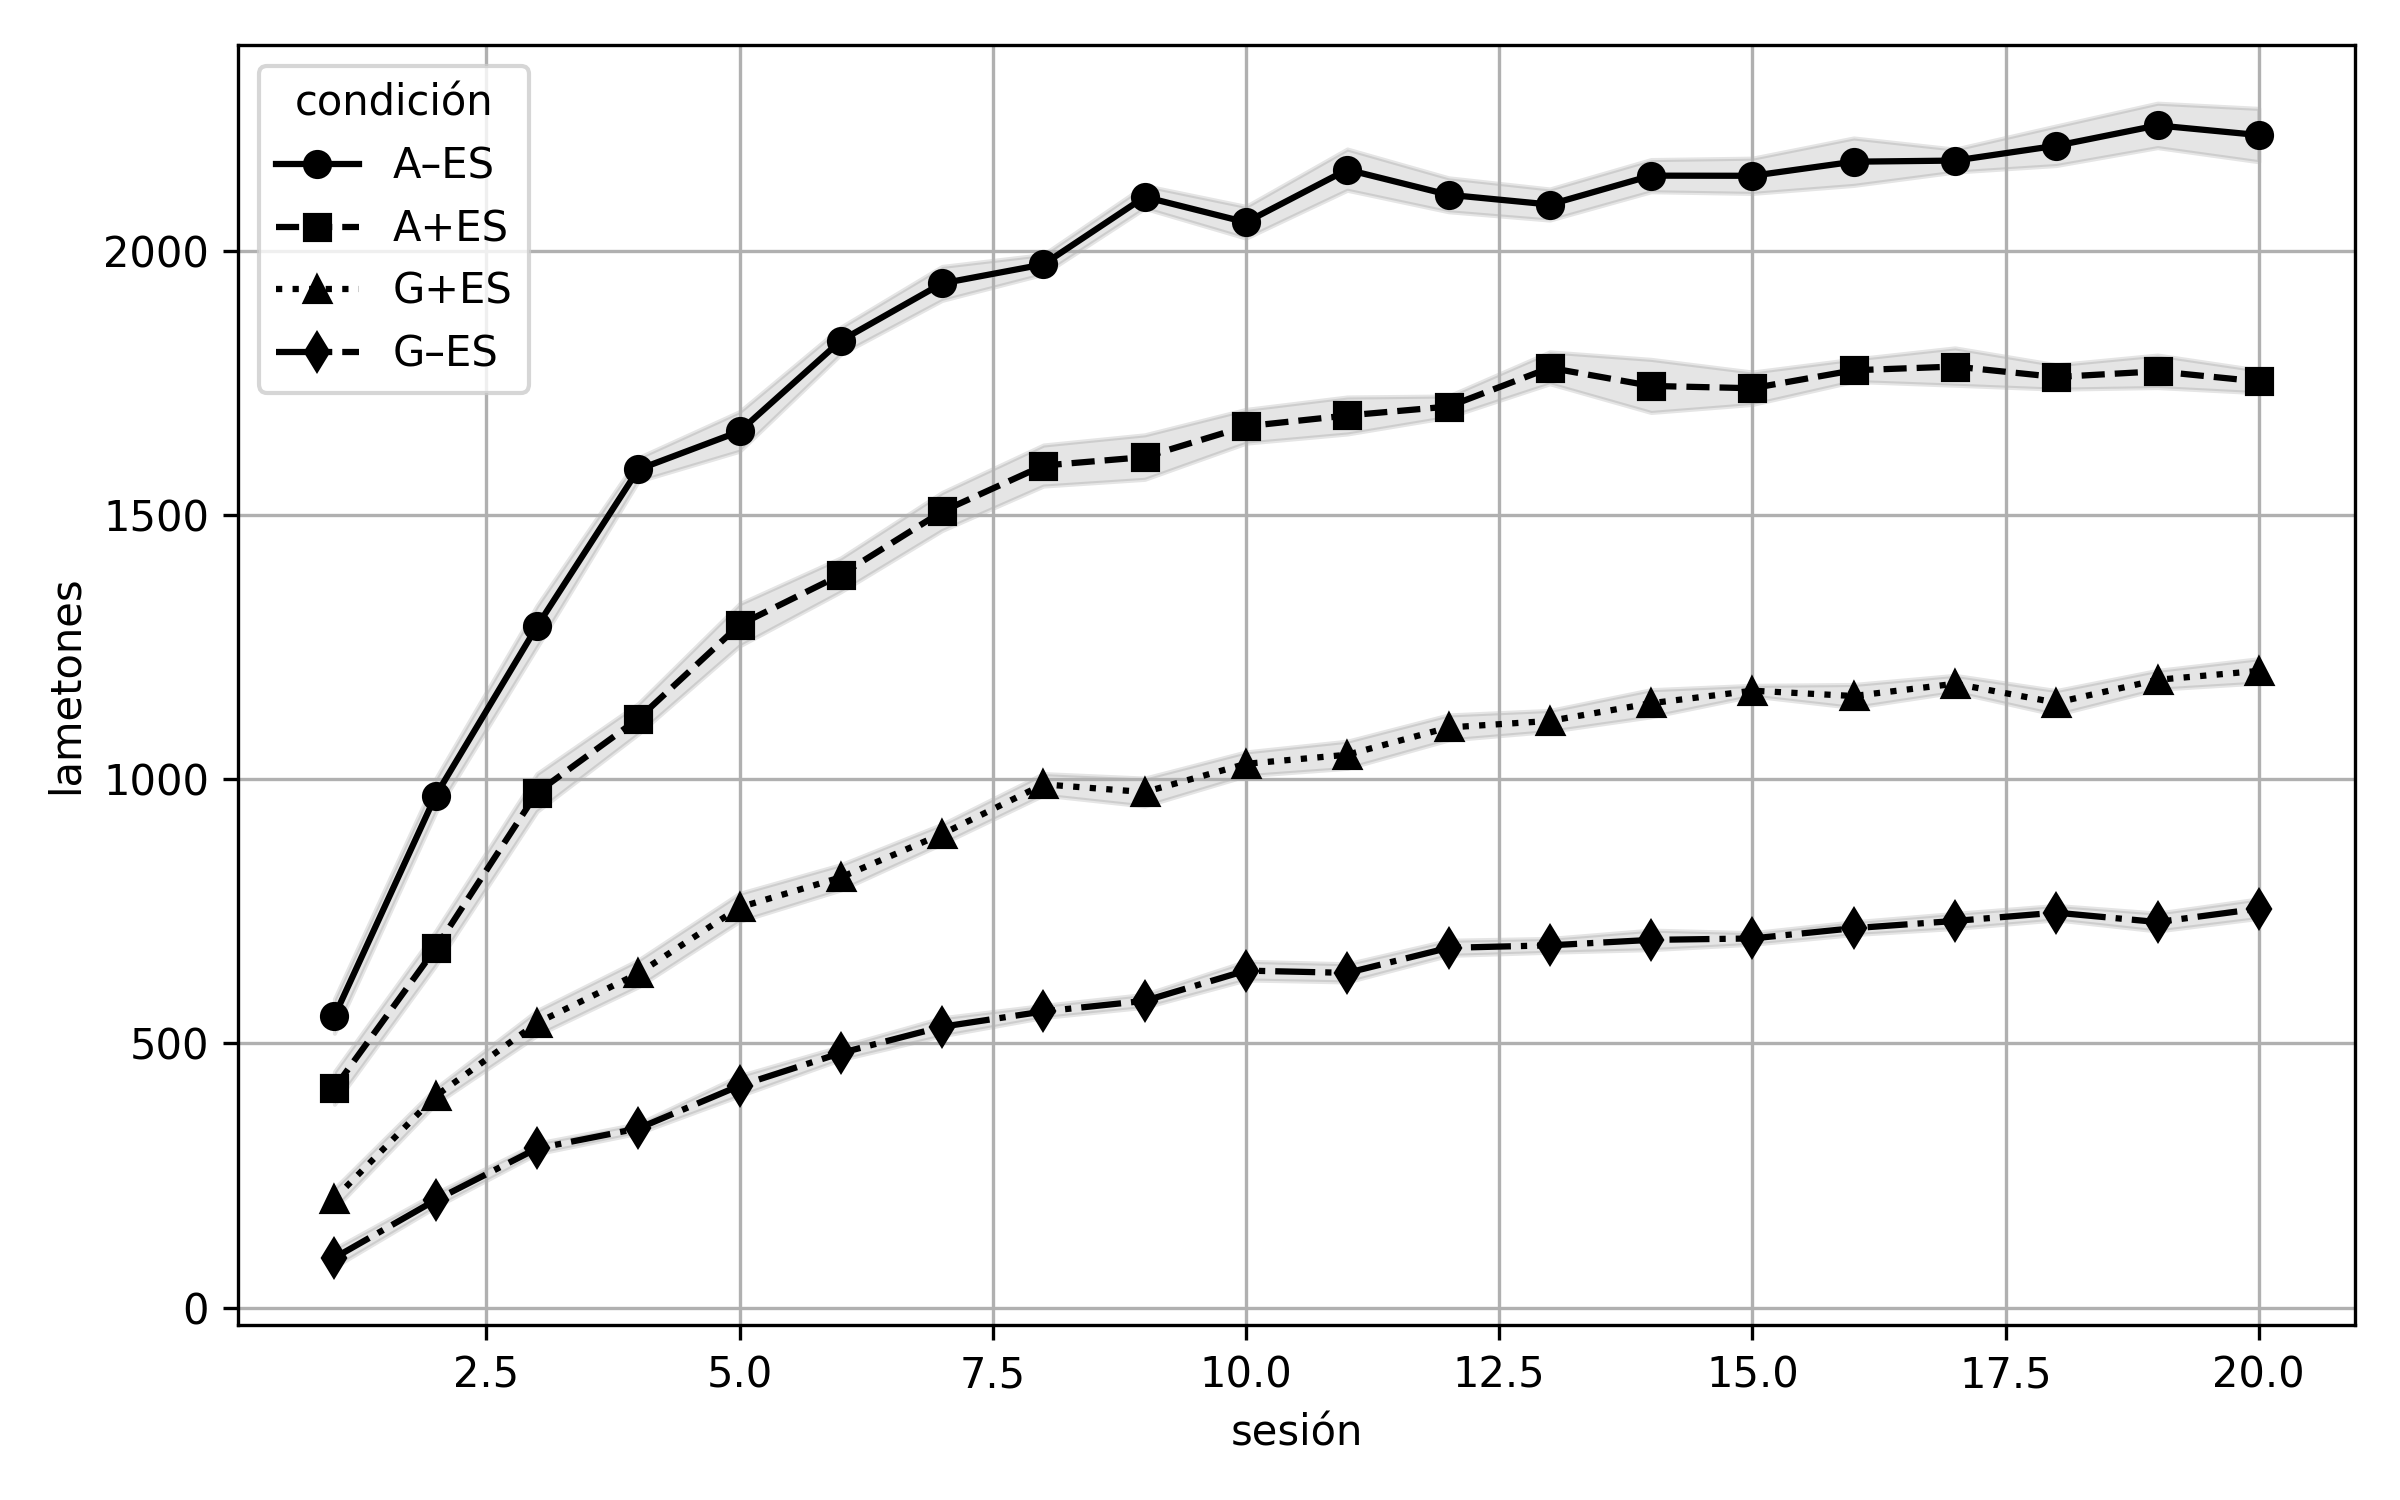
\includegraphics[width=0.45\textwidth]{figura1.png}
\end{figure}

\begin{figure}[H]
\begin{doublespace}
\captionsetup{labelfont=bf, labelsep=none}    
\caption{\textit{\protect\\Distribución individual (boxplots) de lametones en el bloque final de sesiones (16–20)}}
\label{fig:figura2}
\end{doublespace}
\centering
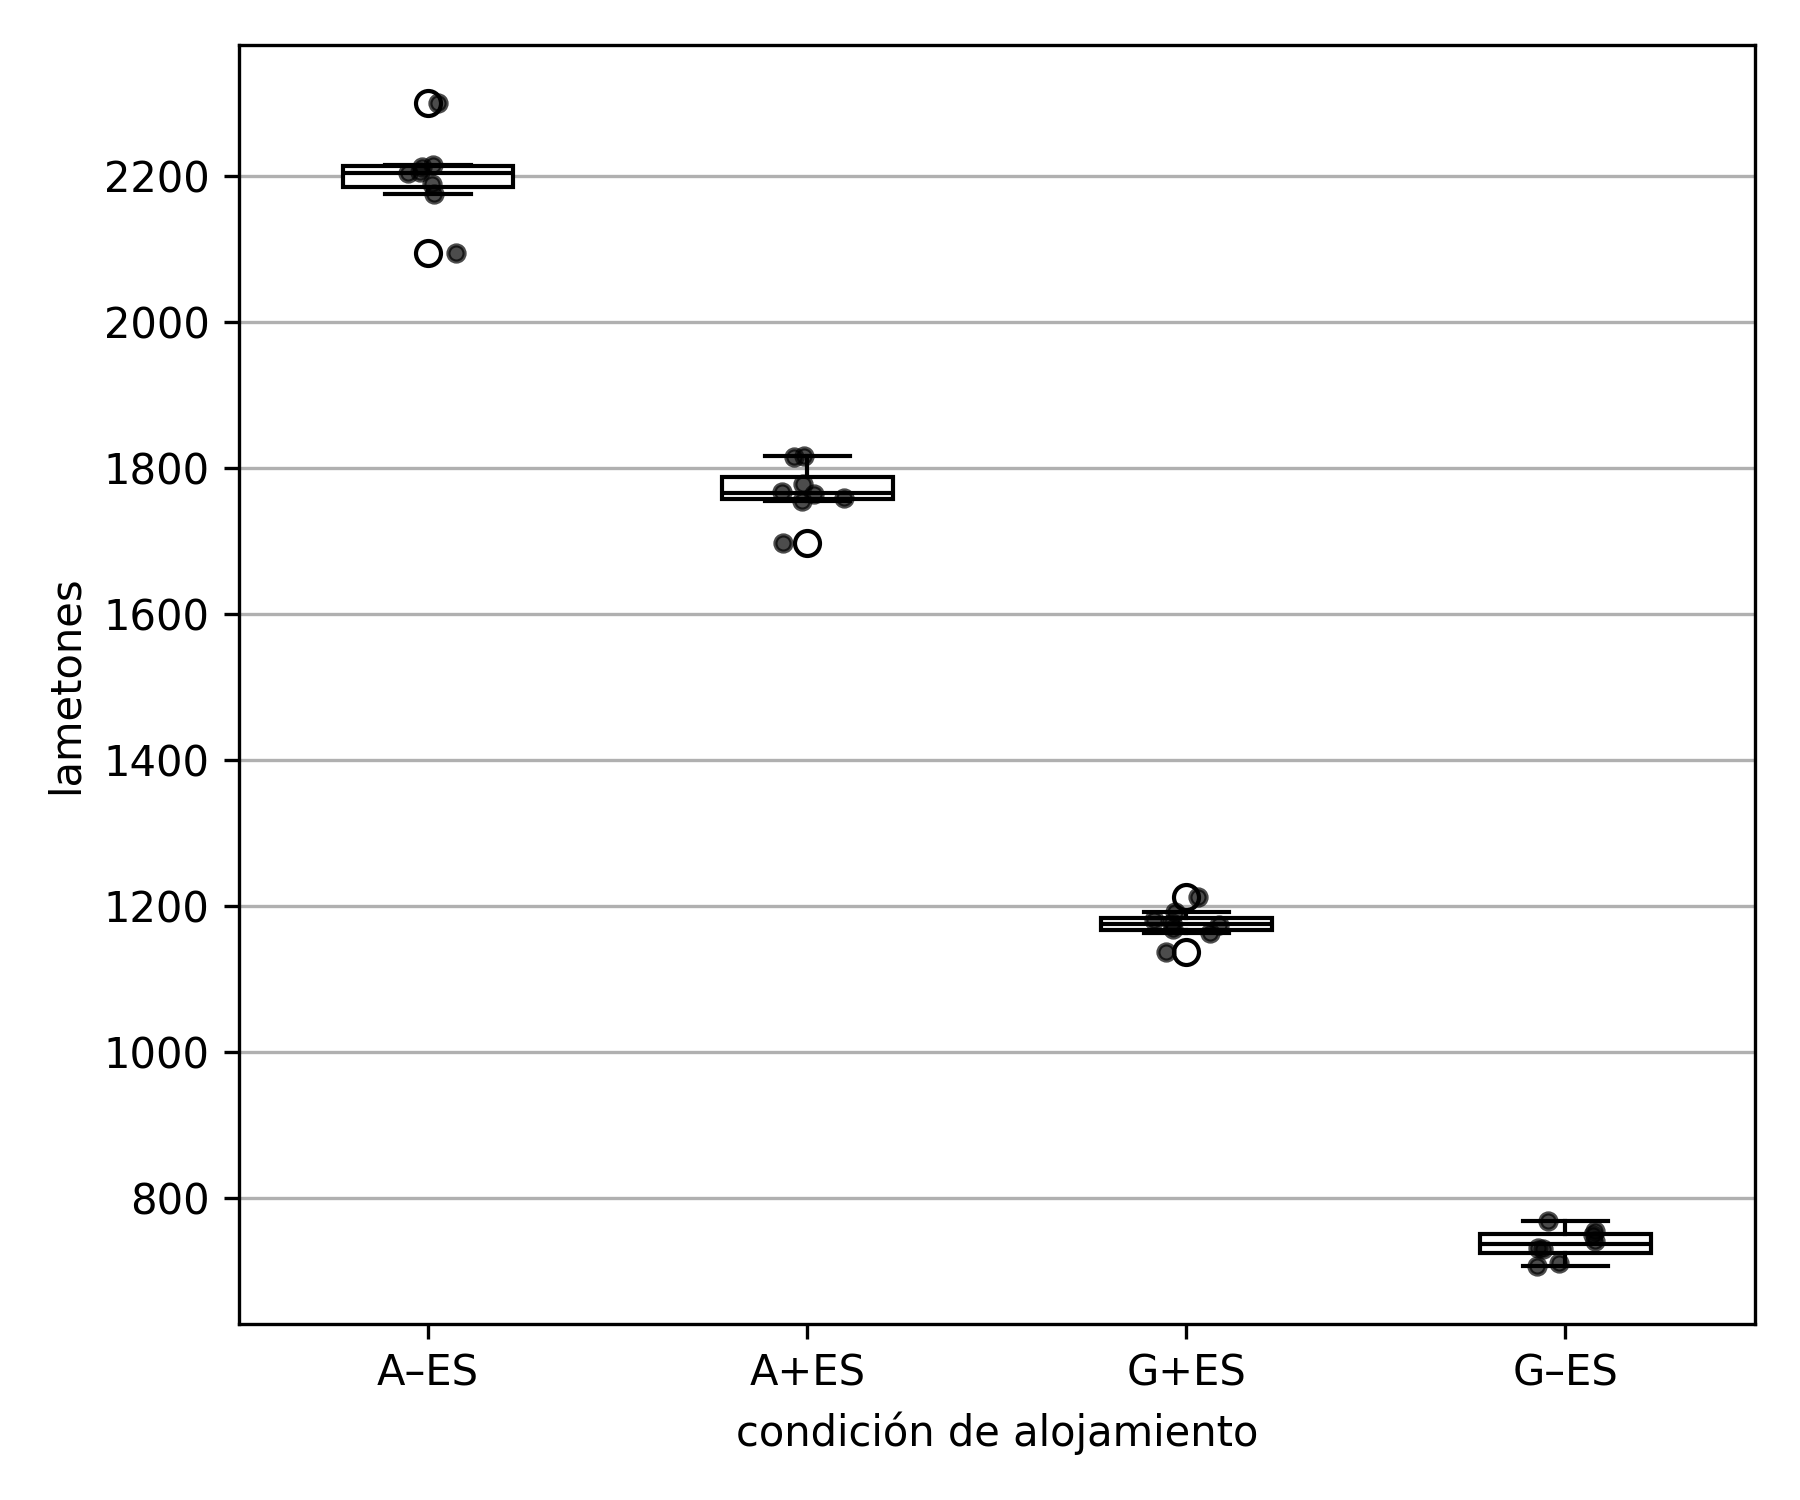
\includegraphics[width=0.45\textwidth]{figura2.png}
\end{figure}


\section{Discusión}

El objetivo de este trabajo es determinar cómo la combinación de privación social y estímulos físicos modula la polidipsia inducida por programa (PIP) y, por extensión, dilucidar si esta conducta adjuntiva puede entenderse como una estrategia de afrontamiento ante un estado emocional alterado. El patrón esperado de resultados, con una mayor expresión de la PIP en la condición de aislamiento sin estimulación sensorial, seguida por el aislamiento con estimulación, el grupo con estimulación y, finalmente, el grupo sin estimulación sensorial, respaldaría la hipótesis inicial: la privación social extrema favorecería la aparición de la PIP, la estimulación sensorial en solitario la atenuaría solo parcialmente y la convivencia social actuaría como amortiguador más potente que cualquier elemento de estimulación sensorial.

Estos resultados proyectados se inscriben en la tradición inaugurada por \citet{Falk1961}, que interpretó la PIP como una actividad desplazada provocada por la incertidumbre generada por el programa de comida. \citet{Staddon1977} refinó esa idea al proponer que las conductas adjuntivas emergen en un estado motivacional intermedio en el que el animal, incapaz de predecir el reforzador, canaliza la activación hacia actividades alternativas. En contraste, el modelo de reforzamiento por contigüidad de \citet{Killeen2013} explica la PIP como el simple resultado del fortalecimiento operante de cualquier respuesta que aparezca lo bastante próxima al pellet. El patrón de datos que se anticipa aquí —máxima PIP bajo aislamiento y mínima en grupo sin estimulación sensorial— sugiere que, aunque la contigüidad temporal contribuye a la consolidación, la motivación emocional impone un techo superior: la conducta no se multiplica indefinidamente, sino que se regula por la necesidad de afrontamiento que impone el contexto.

Aunque el presente diseño prioriza una lectura emocional de la PIP, conviene matizar que ello no excluye la influencia determinante de la entrega del reforzador. De hecho, como han señalado numerosos estudios \citep{Pellon2004}, la PIP solo emerge bajo condiciones específicas de reforzamiento intermitente, y desaparece si se elimina la entrega de alimento, lo que indica que la comida actúa como condición necesaria —aunque no suficiente— para el mantenimiento de la conducta. La teoría del trazo de proximidad formulada por \citet{Killeen2013} sostiene que cualquier conducta que ocurra lo bastante próxima al reforzador tiende a fortalecerse, incluso sin contingencia causal directa. Esta explicación resulta consistente con la topografía temporal de la PIP, que se concentra tras la dispensación del pellet. No obstante, los resultados esperados en este estudio —especialmente la modulación sistemática de la PIP por factores sociales y sensoriales— sugieren que dicha contigüidad no opera en el vacío, sino que su eficacia depende del estado emocional y del contexto ambiental del animal. Es plausible, por tanto, considerar una explicación integradora en la que el reforzador actúe como disparador contingente y la vulnerabilidad emocional determine la probabilidad de consolidación del patrón adjuntivo. En este sentido, la comida no solo refuerza respuestas previas por proximidad, sino que adquiere saliencia motivacional anormal en sujetos con sistemas de afrontamiento alterados, como ocurre tras aislamiento social o privación afectiva.

La lectura emocional cobra fuerza si se compara con el estudio de \citet{FuentesVerdugo2023}. Estos autores describieron una mayor PIP en cajas hogar enriquecidas social y físicamente, concluyendo que la conducta no mitiga el estrés. Sin embargo, esa observación puede entenderse a la luz de lo que algunos autores han descrito como un efecto paradójico del enriquecimiento, consistente en que un historial de alta estimulación puede incrementar la sensibilidad a la frustración cuando se interrumpe el acceso a ciertos estímulos predecibles. Esta idea se alinea con lo señalado por \citet{Wurbel2001}, quien advierte que los efectos del enriquecimiento no son lineales y dependen del historial ambiental del animal. Nuestro diseño diferencia la estimulación sensorial de la social y predice que el enriquecimiento físico sin soporte social eleva la PIP (A+ES), mientras que la vida en grupo sin sobreestimulación (G--ES) la suprime en gran medida. De confirmarse, el hallazgo revelaría que los objetos enriquecedores no son intrínsecamente protectores; su efecto depende del historial social y del grado de activación basal.

La literatura sobre aislamiento respalda esta interpretación. \citet{Fone2008} documentaron que la separación postdestete incrementa ansiedad, impulsividad y conductas repetitivas, acompañadas de hiperreactividad dopaminérgica mesolímbica. \citet{Branchi2006} mostraron que un enriquecimiento social temprano puede, paradójicamente, aumentar la ansiedad adulta cuando el animal es evaluado sin compañeros, lo que subraya la importancia del contexto social actual. \citet{Robbins1989} observaron que ratas aisladas exhiben orientación reforzadora exagerada, fenómeno que se alinea con la hipersensibilidad al valor incentivo que presumiblemente impulsa la PIP. Más recientemente, \citet{Arakawa2018} revisó la reorganización de los circuitos emocionales tras privación social y destacó la vulnerabilidad de la corteza prefrontal medial, clave para la inhibición de respuestas. Por tanto, el aislamiento prolongado no solo genera estrés, sino que reconfigura la codificación de saliencia, de modo que la contigüidad temporal propuesta por \citet{Killeen2013} gana peso precisamente porque el estímulo alimento se vuelve anormalmente atractivo.

El análisis conjunto de las entradas al comedero y la actividad locomotora añadiría matices a esta lectura. El escaso efecto esperado sobre las entradas indica que la motivación primaria por la comida permanece relativamente estable entre grupos; es la conducta adjuntiva la que fluctúa, lo que respalda su carácter de afrontamiento. La actividad locomotora, mayor en condiciones de aislamiento, podría reflejar un estado de activación general elevado, pero debe interpretarse con cautela. \citet{seibenhener2015use} han mostrado que el enriquecimiento ambiental puede influir en la locomoción en el test de campo abierto, afectando tanto a la ansiedad como a la exploración. Si en nuestro protocolo los grupos A+ES y G+ES alcanzaran niveles intermedios de cruces de zona, ello sugeriría que la locomoción responde tanto a la activación emocional como a la exploración facilitada por los objetos.

Las limitaciones del estudio merecen atención. En primer lugar, la estimulación sensorial se limitaría a túneles y objetos manipulables; variantes más cognitivas (laberintos, rompecabezas) podrían modular la PIP de otro modo. Segundo, la muestra incluiría solo machos Wistar; se sabe que las hembras pueden mostrar perfiles de afrontamiento distintos y que la sensibilidad a la privación social es sexo-dependiente. Tercero, la ausencia de biomarcadores —corticosterona plasmática, expresión de fosfo-CREB en núcleo accumbens— impide vincular directamente la conducta con la carga fisiológica de estrés. Cuarto, el tamaño muestral ($n = 8$ por grupo) es adecuado para detectar efectos grandes ($\eta^2_p > .25$), pero podría subestimar interacciones sutiles.

Futuras investigaciones deberían incorporar hembras y analizar posibles interacciones sexo × ambiente, así como profundizar en el papel de los mecanismos neuroendocrinos —en particular la actividad del eje hipotalámico-hipofisario-adrenal (HPA)— y su relación con la desregulación socioemocional, en la medida en que podrían contribuir a la vulnerabilidad frente a conductas compulsivas, tal como sugiere \citet{MartinGonzalez2022}. Además, sería pertinente explorar versiones de enriquecimiento cognitivo y social dinámico, y emplear procedimientos de extinción y reinstalación para evaluar la persistencia de la PIP bajo cambios de contexto, y considerar también el uso de programas de tiempo variable, con el fin de intensificar la incertidumbre del refuerzo y analizar su impacto sobre la expresión de la PIP.


Finalmente, conviene insistir en la limitación que supone la exclusión del sexo como variable experimental. Aunque se ha justificado históricamente por la variabilidad hormonal en hembras, esta práctica ha contribuido a un sesgo de género en la investigación básica. Las diferencias sexo-dependientes en los mecanismos de afrontamiento y en la sensibilidad al estrés social están bien documentadas \citep{Bowman2006, Barha2011}, y su omisión puede restringir la validez ecológica y generalización de los hallazgos. La incorporación sistemática del sexo como factor debe considerarse una prioridad en futuros diseños experimentales.

Desde una perspectiva traslacional, la polidipsia inducida por programa (PIP) se ha propuesto como un modelo animal útil para el estudio de la compulsividad, al presentar características clave como la repetitividad, la descontextualización funcional y la resistencia a la extinción. \citet{Moreno2012} destacan su valor para explorar los mecanismos neuroendocrinos y neurofarmacológicos implicados en trastornos del espectro obsesivo-compulsivo, la esquizofrenia o el abuso de sustancias. En un enfoque más amplio, \citet{Fineberg2010} subrayan la importancia de los modelos animales para caracterizar dimensiones transdiagnósticas como la compulsividad e impulsividad, y abogan por su uso para entender la psicopatología subyacente a estos fenotipos, aunque sin referirse explícitamente al paradigma de la PIP.

En este marco, cabe plantearse también si la estimulación sensorial actúa como un factor que incrementa la compulsividad o, más bien, como un disparador diagnóstico que permite hacerla visible. Es posible que ciertos individuos, particularmente aquellos con una vulnerabilidad previa derivada del aislamiento, presenten una propensión latente a respuestas compulsivas que solo se manifiestan cuando el entorno ofrece oportunidades para su expresión. Desde esta perspectiva, la estimulación sensorial no induciría directamente la PIP, sino que funcionaría como catalizador o amplificador de un patrón ya presente. Esta interpretación invita a repensar el valor del enriquecimiento ambiental no solo como modulador del bienestar, sino también como herramienta exploratoria para revelar diferencias individuales en la sensibilidad emocional al entorno.

En conjunto, los resultados previstos sugerirían esta visión funcional de la PIP como forma de autorregulación emocional más que como conducta estereotipada o producto mecánico del reforzamiento por contigüidad. Su expresión parece modulada por variables contextuales y emocionales, especialmente la privación social, y se ve matizada por el tipo de estimulación sensorial disponible. Distinguir entre enriquecimiento sensorial y social permite abordar la paradoja de que ciertos elementos diseñados para promover el bienestar puedan, en determinadas condiciones, amplificar respuestas disfuncionales. El presente trabajo contribuye así a refinar el marco conceptual desde el que se estudia la compulsividad en modelos animales y a proponer una vía experimental sensible a la interacción entre vulnerabilidad emocional y condiciones ambientales.


\bibliographystyle{apalike}
\bibliography{tfg}

\end{multicols}

\end{document}
